%
% randkarten.tex -- template for standalon tikz images
%
% (c) 2025 Prof Dr Andreas Müller, OST Ostschweizer Fachhochschule
%
\documentclass[tikz]{standalone}
\usepackage{amsmath}
\usepackage{times}
\usepackage{txfonts}
\usepackage{pgfplots}
\usepackage{csvsimple}
\usetikzlibrary{arrows,intersections,math}
\definecolor{darkred}{rgb}{0.8,0,0}
\begin{document}
\def\skala{1}
\begin{tikzpicture}[>=latex,thick,scale=\skala]

\begin{scope}[yshift=8cm]
\node at (0,0) {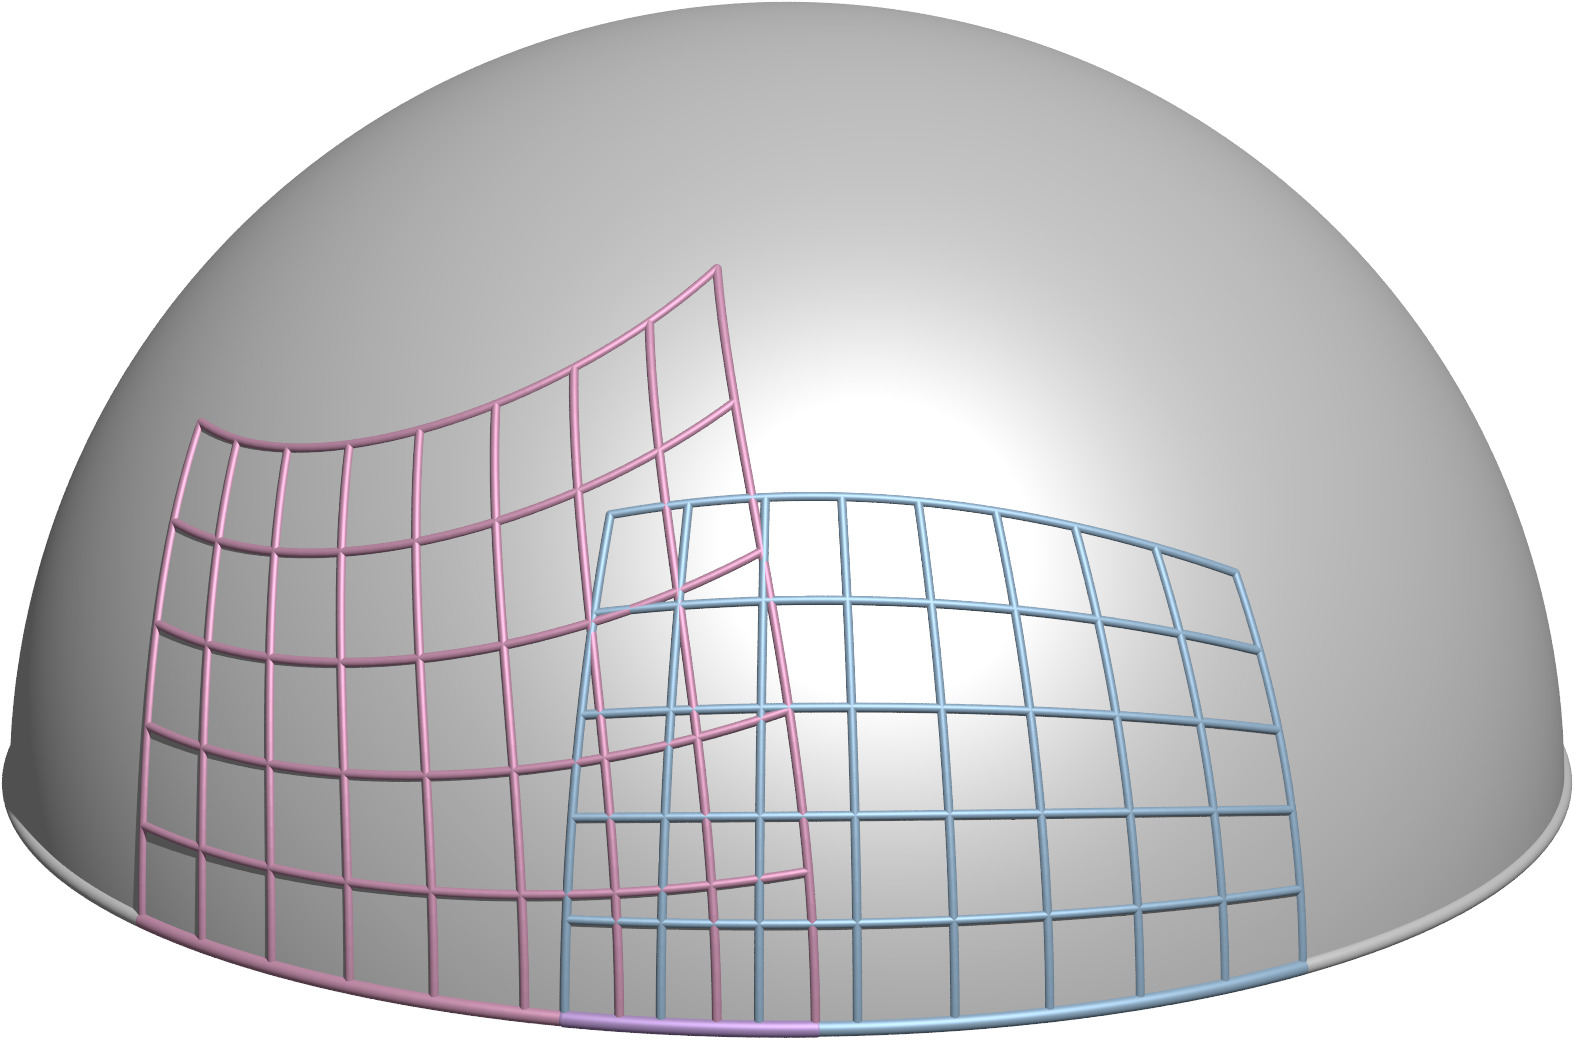
\includegraphics[width=7cm]{randkarten.jpg}};
\draw[->] (-1.8,-2.3) -- ++(-1.4,-3.0);
\node at (-2.5,-3.8) [left] {$\varphi_\alpha$};
\draw[->] (1.8,-2.3) -- ++(1.4,-3.0);
\node at (2.5,-3.8) [right] {$\varphi_\beta$};
\node at (0,2) {$M$};
\node at (3.1,-2) {$\partial M$};
\node at (-1.5,-0.9) {$U_\alpha$};
\node at (-2.4,-2.3) {$\partial U_\alpha$};
\node at (0.9,-1.1) {$U_\beta$};
\node at (1.0,-2.5) {$\partial U_\beta$};
\end{scope}

\begin{scope}[xshift=-3.3cm]
\fill[color=darkred!20] (-2,0) rectangle (2,2.5);
\foreach \x in {-2,-1.5,...,2}{
	\draw[color=darkred] ({\x},0) -- ++(0,2.5);
}
\foreach \y in {0.5,1,...,2.5}{
	\draw[color=darkred] (-2,{\y}) -- ++(4,0);
}
\draw[->] (-2.5,-0.3) -- (-2.5,3.2) coordinate[label={right:$x^n$}];
\draw[->] (-2.6,0) -- (2.9,0) coordinate[label={$x^1$}];
\node at (-1.5,2.5) [above] {$\varphi_\alpha(U_\alpha)$};
\node at (0,0) [below] {$\varphi_\alpha(\partial U_\alpha)$};
\draw[color=darkred,line width=2.0pt] (-2,0) -- (2,0);
\end{scope}

\begin{scope}[xshift=3.3cm]
\fill[color=blue!20] (-2,0) rectangle (2,2.5);
\foreach \x in {-2,-1.5,...,2}{
	\draw[color=blue] ({\x},0) -- ++(0,2.5);
}
\foreach \y in {0.5,1,...,2.5}{
	\draw[color=blue] (-2,{\y}) -- ++(4,0);
}
\draw[->] (-2.5,-0.3) -- (-2.5,3.2) coordinate[label={right:$x^n$}];
\draw[->] (-2.6,0) -- (2.9,0) coordinate[label={$x^1$}];
\node at (1.5,2.5) [above] {$\varphi_\beta(U_\beta)$};
\node at (0,0) [below] {$\varphi_\beta(\partial U_\beta)$};
\draw[color=blue,line width=2.0pt] (-2,0) -- (2,0);
\end{scope}

\end{tikzpicture}
\end{document}

